
%% bare_jrnl.tex
%% V1.4b
%% 2015/08/26
%% by Michael Shell
%% see http://www.michaelshell.org/
%% for current contact information.
%%
%% This is a skeleton file demonstrating the use of IEEEtran.cls
%% (requires IEEEtran.cls version 1.8b or later) with an IEEE
%% journal paper.
%%
%% Support sites:
%% http://www.michaelshell.org/tex/ieeetran/
%% http://www.ctan.org/pkg/ieeetran
%% and
%% http://www.ieee.org/

%%*************************************************************************
%% Legal Notice:
%% This code is offered as-is without any warranty either expressed or
%% implied; without even the implied warranty of MERCHANTABILITY or
%% FITNESS FOR A PARTICULAR PURPOSE!
%% User assumes all risk.
%% In no event shall the IEEE or any contributor to this code be liable for
%% any damages or losses, including, but not limited to, incidental,
%% consequential, or any other damages, resulting from the use or misuse
%% of any information contained here.
%%
%% All comments are the opinions of their respective authors and are not
%% necessarily endorsed by the IEEE.
%%
%% This work is distributed under the LaTeX Project Public License (LPPL)
%% ( http://www.latex-project.org/ ) version 1.3, and may be freely used,
%% distributed and modified. A copy of the LPPL, version 1.3, is included
%% in the base LaTeX documentation of all distributions of LaTeX released
%% 2003/12/01 or later.
%% Retain all contribution notices and credits.
%% ** Modified files should be clearly indicated as such, including  **
%% ** renaming them and changing author support contact information. **
%%*************************************************************************


% *** Authors should verify (and, if needed, correct) their LaTeX system  ***
% *** with the testflow diagnostic prior to trusting their LaTeX platform ***
% *** with production work. The IEEE's font choices and paper sizes can   ***
% *** trigger bugs that do not appear when using other class files.       ***                          ***
% The testflow support page is at:
% http://www.michaelshell.org/tex/testflow/



\documentclass[journal]{IEEEtran}
%
% If IEEEtran.cls has not been installed into the LaTeX system files,
% manually specify the path to it like:
% \documentclass[journal]{../sty/IEEEtran}





% Some very useful LaTeX packages include:
% (uncomment the ones you want to load)


% *** MISC UTILITY PACKAGES ***
%
%\usepackage{ifpdf}
% Heiko Oberdiek's ifpdf.sty is very useful if you need conditional
% compilation based on whether the output is pdf or dvi.
% usage:
% \ifpdf
%   % pdf code
% \else
%   % dvi code
% \fi
% The latest version of ifpdf.sty can be obtained from:
% http://www.ctan.org/pkg/ifpdf
% Also, note that IEEEtran.cls V1.7 and later provides a builtin
% \ifCLASSINFOpdf conditional that works the same way.
% When switching from latex to pdflatex and vice-versa, the compiler may
% have to be run twice to clear warning/error messages.






% *** CITATION PACKAGES ***
%
%\usepackage{cite}
% cite.sty was written by Donald Arseneau
% V1.6 and later of IEEEtran pre-defines the format of the cite.sty package
% \cite{} output to follow that of the IEEE. Loading the cite package will
% result in citation numbers being automatically sorted and properly
% "compressed/ranged". e.g., [1], [9], [2], [7], [5], [6] without using
% cite.sty will become [1], [2], [5]--[7], [9] using cite.sty. cite.sty's
% \cite will automatically add leading space, if needed. Use cite.sty's
% noadjust option (cite.sty V3.8 and later) if you want to turn this off
% such as if a citation ever needs to be enclosed in parenthesis.
% cite.sty is already installed on most LaTeX systems. Be sure and use
% version 5.0 (2009-03-20) and later if using hyperref.sty.
% The latest version can be obtained at:
% http://www.ctan.org/pkg/cite
% The documentation is contained in the cite.sty file itself.






% *** GRAPHICS RELATED PACKAGES ***
%
\usepackage{graphicx}

\ifCLASSINFOpdf
  % \usepackage[pdftex]{graphicx}
  % declare the path(s) where your graphic files are
  % \graphicspath{{../pdf/}{../jpeg/}}
  % and their extensions so you won't have to specify these with
  % every instance of \includegraphics
  % \DeclareGraphicsExtensions{.pdf,.jpeg,.png}
\else
  % or other class option (dvipsone, dvipdf, if not using dvips). graphicx
  % will default to the driver specified in the system graphics.cfg if no
  % driver is specified.
  % \usepackage[dvips]{graphicx}
  % declare the path(s) where your graphic files are
  % \graphicspath{{../eps/}}
  % and their extensions so you won't have to specify these with
  % every instance of \includegraphics
  % \DeclareGraphicsExtensions{.eps}
\fi
% graphicx was written by David Carlisle and Sebastian Rahtz. It is
% required if you want graphics, photos, etc. graphicx.sty is already
% installed on most LaTeX systems. The latest version and documentation
% can be obtained at:
% http://www.ctan.org/pkg/graphicx
% Another good source of documentation is "Using Imported Graphics in
% LaTeX2e" by Keith Reckdahl which can be found at:
% http://www.ctan.org/pkg/epslatex
%
% latex, and pdflatex in dvi mode, support graphics in encapsulated
% postscript (.eps) format. pdflatex in pdf mode supports graphics
% in .pdf, .jpeg, .png and .mps (metapost) formats. Users should ensure
% that all non-photo figures use a vector format (.eps, .pdf, .mps) and
% not a bitmapped formats (.jpeg, .png). The IEEE frowns on bitmapped formats
% which can result in "jaggedy"/blurry rendering of lines and letters as
% well as large increases in file sizes.
%
% You can find documentation about the pdfTeX application at:
% http://www.tug.org/applications/pdftex





% *** MATH PACKAGES ***
%
%\usepackage{amsmath}
% A popular package from the American Mathematical Society that provides
% many useful and powerful commands for dealing with mathematics.
%
% Note that the amsmath package sets \interdisplaylinepenalty to 10000
% thus preventing page breaks from occurring within multiline equations. Use:
%\interdisplaylinepenalty=2500
% after loading amsmath to restore such page breaks as IEEEtran.cls normally
% does. amsmath.sty is already installed on most LaTeX systems. The latest
% version and documentation can be obtained at:
% http://www.ctan.org/pkg/amsmath





% *** SPECIALIZED LIST PACKAGES ***
%
%\usepackage{algorithmic}
% algorithmic.sty was written by Peter Williams and Rogerio Brito.
% This package provides an algorithmic environment fo describing algorithms.
% You can use the algorithmic environment in-text or within a figure
% environment to provide for a floating algorithm. Do NOT use the algorithm
% floating environment provided by algorithm.sty (by the same authors) or
% algorithm2e.sty (by Christophe Fiorio) as the IEEE does not use dedicated
% algorithm float types and packages that provide these will not provide
% correct IEEE style captions. The latest version and documentation of
% algorithmic.sty can be obtained at:
% http://www.ctan.org/pkg/algorithms
% Also of interest may be the (relatively newer and more customizable)
% algorithmicx.sty package by Szasz Janos:
% http://www.ctan.org/pkg/algorithmicx




% *** ALIGNMENT PACKAGES ***
%
%\usepackage{array}
% Frank Mittelbach's and David Carlisle's array.sty patches and improves
% the standard LaTeX2e array and tabular environments to provide better
% appearance and additional user controls. As the default LaTeX2e table
% generation code is lacking to the point of almost being broken with
% respect to the quality of the end results, all users are strongly
% advised to use an enhanced (at the very least that provided by array.sty)
% set of table tools. array.sty is already installed on most systems. The
% latest version and documentation can be obtained at:
% http://www.ctan.org/pkg/array


% IEEEtran contains the IEEEeqnarray family of commands that can be used to
% generate multiline equations as well as matrices, tables, etc., of high
% quality.




% *** SUBFIGURE PACKAGES ***
%\ifCLASSOPTIONcompsoc
%  \usepackage[caption=false,font=normalsize,labelfont=sf,textfont=sf]{subfig}
%\else
%  \usepackage[caption=false,font=footnotesize]{subfig}
%\fi
% subfig.sty, written by Steven Douglas Cochran, is the modern replacement
% for subfigure.sty, the latter of which is no longer maintained and is
% incompatible with some LaTeX packages including fixltx2e. However,
% subfig.sty requires and automatically loads Axel Sommerfeldt's caption.sty
% which will override IEEEtran.cls' handling of captions and this will result
% in non-IEEE style figure/table captions. To prevent this problem, be sure
% and invoke subfig.sty's "caption=false" package option (available since
% subfig.sty version 1.3, 2005/06/28) as this is will preserve IEEEtran.cls
% handling of captions.
% Note that the Computer Society format requires a larger sans serif font
% than the serif footnote size font used in traditional IEEE formatting
% and thus the need to invoke different subfig.sty package options depending
% on whether compsoc mode has been enabled.
%
% The latest version and documentation of subfig.sty can be obtained at:
% http://www.ctan.org/pkg/subfig




% *** FLOAT PACKAGES ***
%
%\usepackage{fixltx2e}
% fixltx2e, the successor to the earlier fix2col.sty, was written by
% Frank Mittelbach and David Carlisle. This package corrects a few problems
% in the LaTeX2e kernel, the most notable of which is that in current
% LaTeX2e releases, the ordering of single and double column floats is not
% guaranteed to be preserved. Thus, an unpatched LaTeX2e can allow a
% single column figure to be placed prior to an earlier double column
% figure.
% Be aware that LaTeX2e kernels dated 2015 and later have fixltx2e.sty's
% corrections already built into the system in which case a warning will
% be issued if an attempt is made to load fixltx2e.sty as it is no longer
% needed.
% The latest version and documentation can be found at:
% http://www.ctan.org/pkg/fixltx2e


%\usepackage{stfloats}
% stfloats.sty was written by Sigitas Tolusis. This package gives LaTeX2e
% the ability to do double column floats at the bottom of the page as well
% as the top. (e.g., "\begin{figure*}[!b]" is not normally possible in
% LaTeX2e). It also provides a command:
%\fnbelowfloat
% to enable the placement of footnotes below bottom floats (the standard
% LaTeX2e kernel puts them above bottom floats). This is an invasive package
% which rewrites many portions of the LaTeX2e float routines. It may not work
% with other packages that modify the LaTeX2e float routines. The latest
% version and documentation can be obtained at:
% http://www.ctan.org/pkg/stfloats
% Do not use the stfloats baselinefloat ability as the IEEE does not allow
% \baselineskip to stretch. Authors submitting work to the IEEE should note
% that the IEEE rarely uses double column equations and that authors should try
% to avoid such use. Do not be tempted to use the cuted.sty or midfloat.sty
% packages (also by Sigitas Tolusis) as the IEEE does not format its papers in
% such ways.
% Do not attempt to use stfloats with fixltx2e as they are incompatible.
% Instead, use Morten Hogholm'a dblfloatfix which combines the features
% of both fixltx2e and stfloats:
%
% \usepackage{dblfloatfix}
% The latest version can be found at:
% http://www.ctan.org/pkg/dblfloatfix




%\ifCLASSOPTIONcaptionsoff
%  \usepackage[nomarkers]{endfloat}
% \let\MYoriglatexcaption\caption
% \renewcommand{\caption}[2][\relax]{\MYoriglatexcaption[#2]{#2}}
%\fi
% endfloat.sty was written by James Darrell McCauley, Jeff Goldberg and
% Axel Sommerfeldt. This package may be useful when used in conjunction with
% IEEEtran.cls'  captionsoff option. Some IEEE journals/societies require that
% submissions have lists of figures/tables at the end of the paper and that
% figures/tables without any captions are placed on a page by themselves at
% the end of the document. If needed, the draftcls IEEEtran class option or
% \CLASSINPUTbaselinestretch interface can be used to increase the line
% spacing as well. Be sure and use the nomarkers option of endfloat to
% prevent endfloat from "marking" where the figures would have been placed
% in the text. The two hack lines of code above are a slight modification of
% that suggested by in the endfloat docs (section 8.4.1) to ensure that
% the full captions always appear in the list of figures/tables - even if
% the user used the short optional argument of \caption[]{}.
% IEEE papers do not typically make use of \caption[]'s optional argument,
% so this should not be an issue. A similar trick can be used to disable
% captions of packages such as subfig.sty that lack options to turn off
% the subcaptions:
% For subfig.sty:
% \let\MYorigsubfloat\subfloat
% \renewcommand{\subfloat}[2][\relax]{\MYorigsubfloat[]{#2}}
% However, the above trick will not work if both optional arguments of
% the \subfloat command are used. Furthermore, there needs to be a
% description of each subfigure *somewhere* and endfloat does not add
% subfigure captions to its list of figures. Thus, the best approach is to
% avoid the use of subfigure captions (many IEEE journals avoid them anyway)
% and instead reference/explain all the subfigures within the main caption.
% The latest version of endfloat.sty and its documentation can obtained at:
% http://www.ctan.org/pkg/endfloat
%
% The IEEEtran \ifCLASSOPTIONcaptionsoff conditional can also be used
% later in the document, say, to conditionally put the References on a
% page by themselves.




% *** PDF, URL AND HYPERLINK PACKAGES ***
%
%\usepackage{url}
% url.sty was written by Donald Arseneau. It provides better support for
% handling and breaking URLs. url.sty is already installed on most LaTeX
% systems. The latest version and documentation can be obtained at:
% http://www.ctan.org/pkg/url
% Basically, \url{my_url_here}.




% *** Do not adjust lengths that control margins, column widths, etc. ***
% *** Do not use packages that alter fonts (such as pslatex).         ***
% There should be no need to do such things with IEEEtran.cls V1.6 and later.
% (Unless specifically asked to do so by the journal or conference you plan
% to submit to, of course. )


% correct bad hyphenation here
\hyphenation{op-tical net-works semi-conduc-tor}


\begin{document}
%
% paper title
% Titles are generally capitalized except for words such as a, an, and, as,
% at, but, by, for, in, nor, of, on, or, the, to and up, which are usually
% not capitalized unless they are the first or last word of the title.
% Linebreaks \\ can be used within to get better formatting as desired.
% Do not put math or special symbols in the title.
\title{Delivering reliable software in the European scientific arena: evolution of methodologies and new trend analysis}
%\title{15 years of European scientific software development: evolution and methodologies}

%
%
% author names and IEEE memberships
% note positions of commas and nonbreaking spaces ( ~ ) LaTeX will not break
% a structure at a ~ so this keeps an author's name from being broken across
% two lines.
% use \thanks{} to gain access to the first footnote area
% a separate \thanks must be used for each paragraph as LaTeX2e's \thanks
% was not built to handle multiple paragraphs
%

\author{Michael~Shell,~\IEEEmembership{Member,~IEEE,}
        John~Doe,~\IEEEmembership{Fellow,~OSA,}
        and~Jane~Doe,~\IEEEmembership{Life~Fellow,~IEEE}% <-this % stops a space
\thanks{M. Shell was with the Department
of Electrical and Computer Engineering, Georgia Institute of Technology, Atlanta,
GA, 30332 USA e-mail: (see http://www.michaelshell.org/contact.html).}% <-this % stops a space
\thanks{J. Doe and J. Doe are with Anonymous University.}% <-this % stops a space
\thanks{Manuscript received April 19, 2005; revised August 26, 2015.}}

% note the % following the last \IEEEmembership and also \thanks -
% these prevent an unwanted space from occurring between the last author name
% and the end of the author line. i.e., if you had this:
%
% \author{....lastname \thanks{...} \thanks{...} }
%                     ^------------^------------^----Do not want these spaces!
%
% a space would be appended to the last name and could cause every name on that
% line to be shifted left slightly. This is one of those "LaTeX things". For
% instance, "\textbf{A} \textbf{B}" will typeset as "A B" not "AB". To get
% "AB" then you have to do: "\textbf{A}\textbf{B}"
% \thanks is no different in this regard, so shield the last } of each \thanks
% that ends a line with a % and do not let a space in before the next \thanks.
% Spaces after \IEEEmembership other than the last one are OK (and needed) as
% you are supposed to have spaces between the names. For what it is worth,
% this is a minor point as most people would not even notice if the said evil
% space somehow managed to creep in.



% The paper headers
\markboth{Journal of \LaTeX\ Class Files,~Vol.~14, No.~8, August~2015}%
{Shell \MakeLowercase{\textit{et al.}}: Bare Demo of IEEEtran.cls for IEEE Journals}
% The only time the second header will appear is for the odd numbered pages
% after the title page when using the twoside option.
%
% *** Note that you probably will NOT want to include the author's ***
% *** name in the headers of peer review papers.                   ***
% You can use \ifCLASSOPTIONpeerreview for conditional compilation here if
% you desire.




% If you want to put a publisher's ID mark on the page you can do it like
% this:
%\IEEEpubid{0000--0000/00\$00.00~\copyright~2015 IEEE}
% Remember, if you use this you must call \IEEEpubidadjcol in the second
% column for its text to clear the IEEEpubid mark.



% use for special paper notices
%\IEEEspecialpapernotice{(Invited Paper)}




% make the title area
\maketitle

% As a general rule, do not put math, special symbols or citations
% in the abstract or keywords.
\begin{abstract}
Ever since the Grid technology appeared as the new paradigm of distributed
computing to the current days of Cloud computing models, the continuous need
of new tools and services to match the scientific community requirements was
addressed in Europe by the creation of software development and
e-Infrastructure coordination dedicated projects. This work examines the
evolution of the software engineering methodologies used in past and present
EU-funded software projects to illustrate how the research on software
reliability has progressed in Europe over the last 15 years following the
foundation of the first project in 2001. Concretely, we describe the team
organizational structure, techniques and procedures that guided the Quality
Assurance definitions to deliver quality software. We highlight the challenges
and barriers faced throughout these years and how they were totally or
partially overcomed. To conclude we discuss the future directions of software
Quality Assurance methodologies for the incoming projects.
\end{abstract}

% Note that keywords are not normally used for peerreview papers.
\begin{IEEEkeywords}
software reliability, quality assurance, software metrics, software testing
techniques
\end{IEEEkeywords}






% For peer review papers, you can put extra information on the cover
% page as needed:
% \ifCLASSOPTIONpeerreview
% \begin{center} \bfseries EDICS Category: 3-BBND \end{center}
% \fi
%
% For peerreview papers, this IEEEtran command inserts a page break and
% creates the second title. It will be ignored for other modes.
\IEEEpeerreviewmaketitle



\section{Introduction}
% The very first letter is a 2 line initial drop letter followed
% by the rest of the first word in caps.
%
% form to use if the first word consists of a single letter:
% \IEEEPARstart{A}{demo} file is ....
%
% form to use if you need the single drop letter followed by
% normal text (unknown if ever used by the IEEE):
% \IEEEPARstart{A}{}demo file is ....
%
% Some journals put the first two words in caps:
% \IEEEPARstart{T}{his demo} file is ....
%
% Here we have the typical use of a "T" for an initial drop letter
% and "HIS" in caps to complete the first word.
\IEEEPARstart{I}{n} the European scientific research arena, the analysis of
some of the last decade software development projects depicts a continuous
increase of the prominence and robustness of testing and validation procedures.
The observed trends are aligned with the evolution of the software engineering
techniques (e.g. rise of DevOps practices) over the last years. This is tied to
the parallel advancements in the ICT field (with virtualization and container
technologies) and the appearance of automation and event-response tools. In the
following we introduce a set of European Commission funded projects that go
from 2001 up to now, where the authors of this summary were and are currently
involved. For each project we explain how they addressed the challenge in
software reliability.

\section{Evolution of research on software reliability in EU-projects}
The DataGrid \cite{cordis:datagrid} project (Jan 2001 -- Dec 2003) was devoted
to develop the first European infrastructure for Grid computing. The project
brought together 21 academic and industry partners, coming from 15 different
countries. There were 3 application areas for requirement gathering i.e.
Particle physics, Bioinformatics and Earth observation. The project delivered
their own software distribution, named EDG (EU DataGrid), strongly based on
Globus Middleware Services \cite{globus}. The development organization
consisted in 5 work packages coordinated by an Architecture Task Force, in
charge of the overall design and technical consistency of the developments.
Mainly due to the fact of having no previous experience in such widely
collaborative projects, a big effort was spent trying to sort out the several
challenges arised \cite{datagrid}, namely the 1) communication overhead, as a
result of the large geographical separation of the parties involved in the
development tasks, 2) the evolution of the requirements coming from the user
communities, and 3) the lack of a body of knowledge for academic software
engineering. Hence agile methodologies were being introduced at that time,
through the Agile manifesto \cite{agile-manifesto}, so the project's
development design suffered from the methods, tools, techniques and best
practices that new discipline software engineering has brought along
\cite{agile}. However, the project focused on the experiences and procedures
from open source software projects, such as Linux and Apache, to try reach a
higher maturity level \cite{cmm}.

\begin{figure*}
\centering
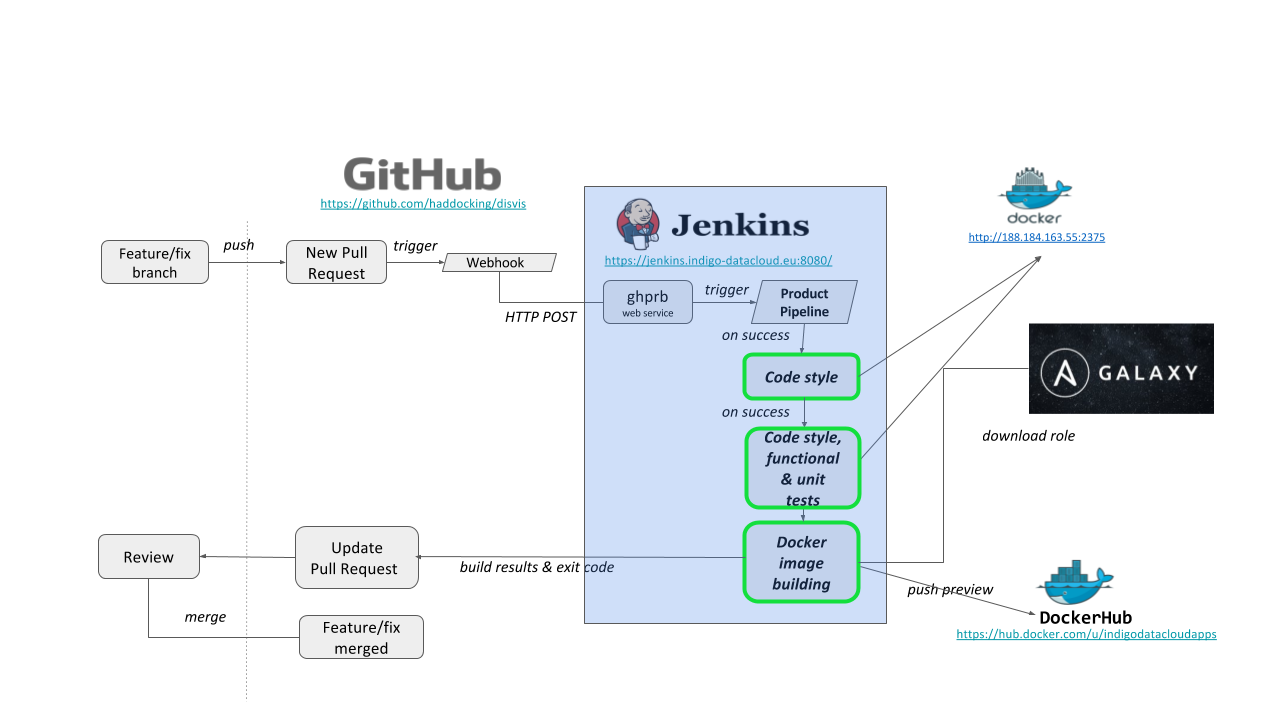
\includegraphics[width=\textwidth]{images/devops.png}
\caption{Continuous Delivery workflow for Docker images.}
\label{fig:fig_CD}
\end{figure*}

The three phases of Enabling Grids for E--sciencE (EGEE, Apr 2004 -- Apr 2010)
\cite{cordis:egee, cordis:egee2, cordis:egee3} projects brought together
scientists and engineers from more than 240 institutions in 45 countries to
provide a seamless Grid infrastructure for e--Science. EGEE--II and EGEE--III
featured the internationalization of the project, embracing worldwide research
institutions and user communities. The software to sustain the increasing
requirements from the diverse scientific communities would need to develop a
rich set of new services while maintaining a sustainable infrastructure for
Grid computing, eventually used by more than 15K researchers and deployed in
over 250 institutions. The {\sl gLite} middleware \cite{glite} was the ultimate
official distribution of EGEE as of 2006, after two years of prototyping and
re--engineering efforts to converge with LHC Computing Grid (LCG--2), Virtual
Data Toolkit (VDT) and Condor \cite{condor} software distributions. The
development team was comprised of more that 80 people from 12 academic and
industrial institutions, that issued more than 10K bugs, 1.7K patches and
defined over 300 tasks tracked by the use of bug/task management tools. The
source code was available at a private, centralized version control system.
The code was not validated by any QA policy, but passed through a manual
certification procedure at the time of the release. This procedure tried to
improve the reliability of the software components by applying a set of
requirements [ref] to be fulfilled at each stage (integration, certification,
pre--production, production), and carried out by different teams. However, from
EGEE--II project, the project adopted the ETICS solution, that aimed to develop
an automatic build system for Grid middleware.

The E-Infrastructure for Testing, Integration and Configuration of Software
\cite{cordis:etics, cordis:etics2} (ETICS, Jan 2006 -- Feb 2010) project aimed
at addressing the challenges in producing quality software in distributed,
collaborative projects like EGEE and its gLite middleware. The framework
integrated different technologies and tools to provide automated configuration,
build and testing capabilities, as well as auto-generated documentation and
software metrics gathering such as Source Lines Of Code (SLOC), complexity and
number of defects/bugs \cite{etics}. ETICS portal was the first automated
service for delivering software products in distributed environments like
Grids.

The European Middleware Initiative (EMI, May 2010 -- Apr 2013)
\cite{cordis:emi} project joined the 4 major Grid middleware providers in
Europe at the time -- {\sl gLite}, {\sl UNICORE}, {\sl ARC} and {\sl dCache} --
to maintain and evolve the middleware focusing on extending the
interoperability in the Grid and improving the reliability of the services. The
ISO/IEC 9126 \cite{iso-9126} standard was used in order to identify a set of
characteristics that needed to be present in the EMI software products and
processes to be able to meet the EMI quality requirements
\cite{emi-quality-model}. For each software characteristic, a set of associated
metrics and Key Performance Indicators (KPIs) were identified and defined in
detail in the EMI Metrics Specification \cite{emi-metrics}. The project
leveraged the {\sl ETICS} service for the development and release management,
as well as for metric tracking, making queries on the collected data to display
them through the chart generation framework.

The EGI--InSPIRE (Integrated Sustainable Pan--European Infrastructure for
Researchers in Europe, May 2010 -- May 2014) project \cite{cordis:egi-inspire}
appeared as the continuation of the EGEE--III project, establishing and
maintaining a sustainable European Grid Infrastructure. EGI--InSPIRE did not
develop any software but maintained a production--ready Grid computing
middleware distribution called {\sl UMD} (Unified Middleware Distribution).
The role of {\sl UMD} was to enforce the fulfilment of a set of quality
criteria definitions \cite{egi-qc} in the software being delivered (i.e.,
{\sl EMI} and {\sl Globus}) \cite{mario}. {\sl UMD} is still being used and
deployed in the European scientific e--Infrastructures under a follow--up
project, the EGI--Engage (Engaging the EGI Community towards an Open Science
Commons) \cite{cordis:egi-engage}. This distribution is currently complemented
by a Cloud--specific one called {\sl CMD} (Cloud Middleware Distribution).

The INDIGO-DataCloud (INtegrating Distributed data Infrastructures for Global
ExplOitation, Apr 2015 -- Sep 2017) \cite{cordis:indigo} is the ultimate
project of software development of the ones reviewed. At the time of writing
the project is succeeding to provide solutions to address the existing gaps in
cloud Platform--as--a--Service (PaaS) and Software-as-a-Service (SaaS) levels,
helping developers, e--Infrastructures and scientific communities to exploit
Cloud computing benefits.

\begin{figure*}
\centering
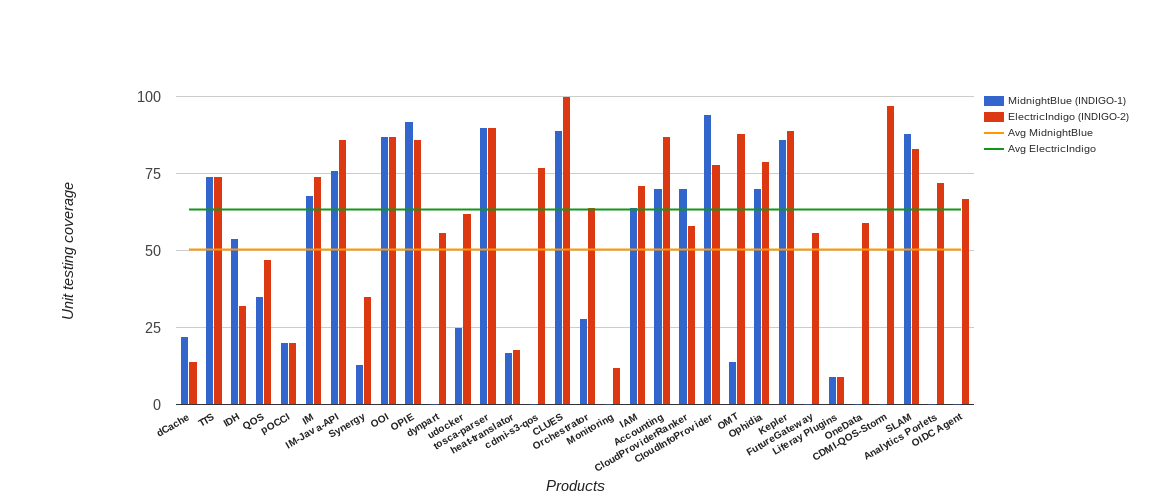
\includegraphics[width=\textwidth]{images/unittest.png}
\caption{Unit testing coverage for the two major INDIGO--DataCloud releases.}
\label{fig:fig_unittest}
\end{figure*}

\section{New Trends in Software Reliability}

The INDIGO--Datacloud project is a reflection of the progress made in software
quality and reliability aspects throughout the past scientific European
experiences. Nevertheless, the project’s Quality Assurance procedures are also
highly influenced by the insights of current big worldwide collaborations of
software development. These collaborations have continuously inspired new
technologies and procedures to increase the robustness and quality of the
software being delivered. In this scenario, the DevOps culture is one of the
major outcomes that has been progressively adopted in the INDIGO--DataCloud
project.

\subsection{DevOps practices}

The DevOps methods emphasize on exercising Quality Assurance techniques to
avoid infrastructure disruption whenever new developments are deployed into
production. The INDIGO--DataCloud project promoted the application of a CI
scenario to enforce the Quality Assurance requirements for any piece of
software being produced within the project. Such environment requires an
automated ready--to--go infrastructure where the different services involved
(source code management platform, automation server) interact with each other
to trigger the quality check execution and return back the exit codes, together
with their outputs. To accomplish this, the project leveraged tightly
integrated open source tools such as GitHub and Jenkins, as well as relying on
Docker container provisioning to speed up the source code validation. This CI
approach is guiding the project’s software development phase throughout the
first and second major releases.

As DevOps suggests, frequent releases positively affects the reliability of the
software. The software updates of INDIGO--DataCloud products taking place since
the second major release are passing through a Continuous Delivery (CD)
pipeline that adds the packaging of the software right after the execution of
the quality checks (as part of the CI). The steps defined within the CD
pipeline differ whether the software is to be distributed in the form of Docker
images or via operating system’s packages. In the latter case an extra
validation step is added, consisting in the product’s deployment using a
Configuration Management (CM) solution. The installation uses the packages
being built in the previous step, which are being uploaded to a testing
repository. In the case of Docker images, the CM is used to build the image
itself, installing and configuring the product before uploading it to the
DockerHub repository \cite{indigo-dockerhub}. Figure \ref{fig:fig_CD} showcases
the workflow followed by the products distributed as Docker images.

\subsection{Software Quality Procedures}

The software quality procedures \cite{indigo-d31} cover: 1) the identification
and description of the \emph{quality requirements} that the software need to
comply with, and 2) the \emph{quality metrics}.

The requirements are applied at early stages in the software development
process, integrated in the Jenkins CI service \cite{indigo-jenkins}, so any
bug or design issue is likely to be detected and corrected promptly. The source
code is publicly available in GitHub repositories under an organization called
{\sl indigo-dc} \cite{indigo-github} to augment the visibility of the product
catalogue, promoting the external contributions and software adoption. In this
regard, the source code is compliant with community de--facto style standards,
selected from the variety of programming languages being used.

\begin{figure}[!t]
\centering
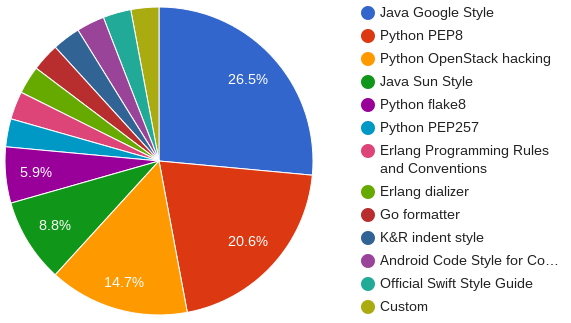
\includegraphics[width=0.5\textwidth]{images/codestyle.png}
\caption{Code style standards followed by INDIGO--DataCloud's software products.}
\label{fig:fig_codestyle}
\end{figure}

Tests are triggered in each build to measure the unit and functional testing
coverage, with a recommended value of 70\% of coverage in the former case. The
documentation of the products is treated as source code, using a markup
language, automatically rendered and uploaded in online repositories
\cite{indigo-gitbook}. Changes in both documentation and source code are
human--reviewed as the last step before merging them into the production
repository. Last but not least, as already seen in the DevOps section, in order
to facilitate the usage of the INDIGO--DataCloud services, they can be deployed
automatically using either Ansible \cite{indigo-ansible} or Puppet
\cite{indigo-puppet} open--source tools.

The evaluation of the software quality is performed by measuring the values of
the metrics and Key Performance Indicators (KPIs) defined based upon the
ISO/IEC 9126 standard. These metrics cover the development, release and
maintenance phases of the software lifecycle. Development and release metrics
are obtained automatically from several sources, such as GitHub and Jenkins CI
service, and graphically displayed as GitHub pages using GrimoireLab framework
\cite{grimoirelab}. Maintenance and user support metrics are collected from the
different sources of data like GGUS \cite{ggus} and Github Issues.

\subsection{Integration, preview and early adoption}

Two pilot infrastructures are at the disposal of developers and scientific
communities involved in the project. The aim of these testbeds is to test the
level of integration between the components involved in the INDIGO--DataCloud
solution and use cases validation, by deploying and executing the applications
with the last stable version of the software.

The released software is also tested in production environments through the
stage--rollout process. Selected resource providers are requested to install
the most updated stable versions of the software, accessed by their users. The
stage--rollout process is key to detect and mitigate issues that could only
appear in production.


\section{Conclusion}

It is a fact that the European software produced for scientific purposes is
evolving to a more sustainable model where the quality and reliability of
software is being prioritized. Recent software engineering insights, such as
DevOps, are gradually being applied as the open--source collaborative tools
evolve, allowing tighter integrations. The focus of the Software Quality
Assurance procedures has been integrated in the development stage, trying to
detect and correct issues early in the software lifecycle. Automation and
metric analysis are at the base of prompt issue solving. However, post--release
validation, such as integration testbeds and the stage--rollout process, are
also needed to strengthen the software reliability for scientific usage.


%\appendices
%\section{Proof of the First Zonklar Equation}
%Appendix one text goes here.
%
%% you can choose not to have a title for an appendix
%% if you want by leaving the argument blank
%\section{}
%Appendix two text goes here.


% use section* for acknowledgment
\section*{Acknowledgment}

The authors would like to thanks European Commission with the various funded
projects.


% Can use something like this to put references on a page
% by themselves when using endfloat and the captionsoff option.
\ifCLASSOPTIONcaptionsoff
  \newpage
\fi



% trigger a \newpage just before the given reference
% number - used to balance the columns on the last page
% adjust value as needed - may need to be readjusted if
% the document is modified later
%\IEEEtriggeratref{8}
% The "triggered" command can be changed if desired:
%\IEEEtriggercmd{\enlargethispage{-5in}}

% references section

% can use a bibliography generated by BibTeX as a .bbl file
% BibTeX documentation can be easily obtained at:
% http://mirror.ctan.org/biblio/bibtex/contrib/doc/
% The IEEEtran BibTeX style support page is at:
% http://www.michaelshell.org/tex/ieeetran/bibtex/
%\bibliographystyle{IEEEtran}
% argument is your BibTeX string definitions and bibliography database(s)
%\bibliography{IEEEabrv,../bib/paper}
%
% <OR> manually copy in the resultant .bbl file
% set second argument of \begin to the number of references
% (used to reserve space for the reference number labels box)
\begin{thebibliography}{1}

\bibitem{cordis:datagrid}
\emph{DataGrid project}, European Community Research and Development
Information Service (CORDIS),
http://cordis.europa.eu/project/rcn/53665\_en.html

\bibitem{globus}
I. Foster and C. Kesselman, \emph{Globus: a Metacomputing Infrastructure
Toolkit}, International Journal of Supercomputer Applications, vol. 11, no. 2,
pp. 115–128, 1997.

\bibitem{datagrid}
L. Momtahan and A. Martin, \emph{e-Science Experiences: Software Engineering
Practice and the EU DataGrid}, in Proc. Asia-Pacific Software Engineering
Conference, Gold Coast, Queensland, Australia, pp. 269-275, IEEE Press,
4-6 Dec. 2002.

\bibitem{agile-manifesto}
\emph{Manifesto for Agile Software Development}, http://agilemanifesto.org

\bibitem{agile}
T. Dingsoyr, \emph{A decade of agile methodologies: Towards explaining agile
software development} in The Journal of Systems and Software, Elsevier Inc,
2012.

\bibitem{cmm}
Paulk et al., \emph{Capability maturity model for software}, Software
Engineering Institute, report CMU/SEI-93-TR-24, ESC-TR-93-177, Feb. 1993.

\bibitem{cordis:egee}
\emph{Enabling Grids for E-sciencE (EGEE)} project, European Community
Research and Development Information Service (CORDIS),
http://cordis.europa.eu/project/rcn/80149\_en.html

\bibitem{cordis:egee2}
\emph{Enabling Grids for E-sciencE-II (EGEE-II)} project, European Community
Research and Development Information Service (CORDIS),
http://cordis.europa.eu/project/rcn/99189\_en.html

\bibitem{cordis:egee3}
\emph{Enabling Grids for E-sciencE-III (EGEE-III)} project, European Community
Research and Development Information Service (CORDIS),
http://cordis.europa.eu/project/rcn/87264\_en.html

\bibitem{glite}
E. Laure et al, \emph{Programming the Grid with gLite}, in Jin, H., Reed, D.A.,
Jiang, W. (eds.) Computational Methods in Science and Technology, vol. 12(1),
pp. 33–45, Scientific Publishers OWN, 2006.

\bibitem{condor}
D. Thain, T. Tannenbaum, M. Livny, \emph{Condor and the grid}, in Grid
Computing: Making the Global Infrastructure a Reality, Chapter 11, pp. 63–70,
Eds. John Wiley \& Sons Inc., 2002.

\bibitem{cordis:etics}
\emph{E-Infrastructure for Testing, Integration and Configuration of Software
(ETICS)} project, European Community Research and Development Information
Service (CORDIS), http://cordis.europa.eu/project/rcn/80138\_en.html

\bibitem{cordis:etics2}
\emph{E-Infrastructure for Testing, Integration and Configuration of Software -
Phase 2 (ETICS 2)} project, European Community Research and Development
Information Service (CORDIS),
http://cordis.europa.eu/project/rcn/86604\_en.html

\bibitem{etics}
A. Di Meglio, M.-E.Bégin, P. Couvares, E. Ronchieri, E. Takacs, \emph{ETICS:
the international software engineering service for the grid}, in Journal of
Physics: Conference Series, Vol. 119, N. 4, IOP Publishing Ltd, 2008.

\bibitem{cordis:emi}
\emph{European Middleware Initiative (EMI)} project, European Community
Research and Development Information Service (CORDIS),
http://cordis.europa.eu/project/rcn/95311\_en.html

\bibitem{iso-9126}
\emph{ISO/IEC 9126 Software Engineering - Product Quality}, International
Organization for Standarization, https://www.iso.org/standard/22749.html

\bibitem{emi-metrics}
\emph{EMI Metrics Specification}, https://goo.gl/CCtY7x


\bibitem{emi-quality-model}
\emph{EMI Quality Model}. Available: https://goo.gl/LdS6fL

\bibitem{cordis:egi-inspire}
\emph{European Grid Initiative: Integrated Sustainable Pan-European
Infrastructure for Researchers in Europe (EGI-InSPIRE)} project, European
Community Research and Development Information Service (CORDIS),
http://cordis.europa.eu/project/rcn/95923\_en.html

\bibitem{egi-qc}
\emph{EGI Quality Criteria}. Available: http://egi-qc.github.io/

\bibitem{mario}
M. David et al, \emph{Validation of Grid Middleware for the European Grid
Infrastructure}, in Journal of Grid Computing, vol. 12, issue 3, pp. 543–558,
Springer, 2014.

\bibitem{cordis:egi-engage}
\emph{Engaging the EGI Community towards an Open Science Commons (EGI-ENGAGE)}
project, European Community Research and Development Information Service
(CORDIS), http://cordis.europa.eu/project/rcn/194937\_en.html

\bibitem{cordis:indigo}
\emph{INtegrating Distributed data Infrastructures for Global ExplOitation
(INDIGO-DataCloud)} project, European Community Research and Development
Information Service (CORDIS),
http://cordis.europa.eu/project/rcn/194882\_en.html

\bibitem{indigo-dockerhub}
\emph{INDIGO-DataCloud DockerHub repository},
https://hub.docker.com/u/indigodatacloud

\bibitem{indigo-d31}
\emph{Initial Plan for WP3} INDIGO-DataCloud Deliverable 3.1,
https://www.indigo-datacloud.eu/documents/initial-plan-wp3-d31

\bibitem{indigo-jenkins}
\emph{INDIGO-DataCloud Jenkins CI service},
https://jenkins.indigo-datacloud.eu:8080/

\bibitem{indigo-github}
\emph{INDIGO-DataCloud GitHub Source Code repository},
https://www.github.com/indigo-dc

\bibitem{indigo-gitbook}
\emph{INDIGO-DataCloud GitBook Documentation repository},
https://www.gitbook.com/@indigo-dc

\bibitem{indigo-puppet}
\emph{INDIGO-DataCloud PuppetForge repository},
https://forge.puppet.com/indigodc

\bibitem{indigo-ansible}
\emph{INDIGO-DataCloud Ansible Galaxy repository},
https://galaxy.ansible.com/indigo-dc/

\bibitem{grimoirelab}
\emph{GrimoireLab}, http://grimoirelab.github.io/

\bibitem{ggus}
\emph{Global Grid User Support (GGUS)}, https://www.ggus.eu/

\end{thebibliography}

% biography section
%
% If you have an EPS/PDF photo (graphicx package needed) extra braces are
% needed around the contents of the optional argument to biography to prevent
% the LaTeX parser from getting confused when it sees the complicated
% \includegraphics command within an optional argument. (You could create
% your own custom macro containing the \includegraphics command to make things
% simpler here.)
%\begin{IEEEbiography}[{\includegraphics[width=1in,height=1.25in,clip,keepaspectratio]{mshell}}]{Michael Shell}
% or if you just want to reserve a space for a photo:

\begin{IEEEbiography}{Michael Shell}
Biography text here.
\end{IEEEbiography}

% if you will not have a photo at all:
\begin{IEEEbiographynophoto}{John Doe}
Biography text here.
\end{IEEEbiographynophoto}

% insert where needed to balance the two columns on the last page with
% biographies
%\newpage

\begin{IEEEbiographynophoto}{Jane Doe}
Biography text here.
\end{IEEEbiographynophoto}

% You can push biographies down or up by placing
% a \vfill before or after them. The appropriate
% use of \vfill depends on what kind of text is
% on the last page and whether or not the columns
% are being equalized.

%\vfill

% Can be used to pull up biographies so that the bottom of the last one
% is flush with the other column.
%\enlargethispage{-5in}



% that's all folks
\end{document}


